\documentclass[a4paper,11pt]{report}
\usepackage{polski}
\usepackage[utf8]{inputenc}
\usepackage{graphicx} % obrazki
\usepackage{fancyvrb} % spacje w verbatim
\usepackage[table]{xcolor}
\usepackage{geometry}
\usepackage{indentfirst}
\usepackage{arydshln}
\usepackage{tikz}
\usepackage{pgfplots}
\pgfplotsset{every tick label/.append style={font=\footnotesize}}
\title{Quicksort}
\author{Rafał Stępień Krzysztof Kotlarz}
\date{\today}
\begin{document}
\renewcommand{\tabcolsep}{10mm}
\newgeometry{tmargin=2cm,bmargin=2cm,lmargin=2cm,rmargin=2cm}

\begin{titlepage}
   \begin{center}
       \vspace*{9cm}
 
       \textbf{\huge{Quicksort - sortowanie szybkie}}
 
       \vspace{1.5cm}
 
       Rafał Stępień | Krzysztof Kotlarz \\
       \vspace{2cm}

 
       Wydział Biologii i Hodowli Zwierząt\\
       Uniwersytet Przyrodniczy we Wrocławiu\\
       Bioinformatyka\\
 
   \end{center}
\end{titlepage}
\newpage
\tableofcontents
\newpage
\chapter{Wprowadzenie}
\hspace{10pt}Quicksort został wynaleziony przez brytyjskiego informatyka Tony'ego Hoare'a i jest jednym z najpopularniejszych algorytmów sortujących. Do dnia dzisiejszego powszechnie używany, jednak ze względu na rekurencyjne działanie, trzeba uważać przy jego stosowaniu i nie można go implementować bezmyślnie, bo może prowadzić to do przepełnienia stosu rekurencji i zablokowania komputera, lub spadku wydajności, jeżeli zapominamy o najgorszym przypadku i w efekcie algorytm nie jest już taki dobry. \\
\\
W przypadku rozważania efektywności algorytmu quicksort bierzemy pod uwagę przede wszystkim dwa przypadki: najlepszy i średni, można jednak wysnuć intuicje dotyczące przypadku najgorszego.
\chapter{Działanie algorytmu}
\section{Ogólny opis działania}
Algorytm jest oparty na technice "dziel i zwyciężaj", którą możemy podzielić na 3 kroki:
\begin{enumerate}
\item \textbf{Dziel} - Tablica $A[]$ jest dzielona na dwie części, takie, że każdy element tablicy pierwszej jest nie większy niż $A[q]$, a każdy element tablicy drugiej jest większy od $A[q]$. Możemy wywnioskować że bardzo ważnym krokiem będzie wybór elementu $A[q]$.
\item \textbf{Zwyciężaj} - Obydwie podtablice są sortowane rekurencyjnymi wywołaniami quicksort.
\item \textbf{Połącz} - Z racji tego, że sortowanie odbywa się w miejscu nie musimy łączyć tablic, ponieważ są one już automatycznie połączone.
\end{enumerate}
\subsubsection{Zalety}
\begin{itemize}
\item \textbf{Sortowanie w miejscu} - zaletą takiego działania jest to, że nie zużywamy dodatkowej pamięci, ponieważ operacje są wykonywane za każdym razem na tej samej liście, nie tworzymy nowej.
\item \textbf{Szybkość średniego przypadku} - jego oczekiwany czas działania wynosi $\theta(nlgn)$, a stałe ukryte pod znakiem $\theta$ są małe.
\item Działa dobrze w środowiskach wykorzystujących \textbf{pamięć wirtualną}
\end{itemize}

\section{Podział tablicy}
Dzięki funkcji def partition następuje podzielenie większych problemów na mniejsze. Wykorzystany zostanie pivot, czyli element który pozwoli wyznaczyć na dwa podproblmy. Elementy na lewo od pivot'a będą od niego mniejsze, zaś po jego prawej stronie, większe.


Procedurę zaczęto od wybrania wartości p, która ma być pivotem wg. jednej z 4 funkcji (wartość ze zbioru znajdująca się na: końcu, początku, w miejscu środkowym lub z losowego miejsca), względem której będzie dokonywany podział. Indeksem pivota zawsze zostaje miejsce będące ostatnią pozycją analizowanego przedziału.


Element $i$-ty to element obecnie poddawany analizie w ciele pętli. natomiast element $j$-ty jest to tzw. border 
w którego miejsce wstawiane będą elementy $i$-te. Ostatecznie border wyznacza miejsce w które trafić ma pivot po wyjściu z pętli oraz miejsce zawierające element posortowany, który znajduje się we właściwym miejscu. Pivot nie zostaje analizowany podczas iteracji


Procedurę zaczynamy zawsze od początku do końca wyznaczonego zbioru. Element $i$-ty zostaje zamieniony z $j$-tym w momencie, gdy i$<$p. Zbiór analizowany jest element po elemencie. Gdy następuje zamiana, element $j$ zostaje przesunięty $+1$. Komórki zaznaczone na szaro to elementy ulegające zamianie w danej iteracji.

\newpage
\begin{table}[h!]
\Large
\centering
\begin{tabular}{|c|c|c|c|c|c|}
\hline
\cellcolor{black!25} &  &  &  &  & \\
\cellcolor{black!25}2 & 8 & 7 & 1 & 3 & 5 \\ \hdashline
i=j&  & &  &  & p\\ \hline
\end{tabular}

\end{table}

Element $i$-ty = 2 jest mniejszy od p$=$5. Zostaje on zamieniony z elementem $j$-tym. W tym przypadku następują zamiana w miejscu.

\begin{table}[h!]
\Large
\centering
\begin{tabular}{|c|c|c|c|c|c|}
\hline
 &  &  &  &  & \\
2 & 8 & 7 & 1 & 3 & 5 \\ \hdashline
 & i=j & &  &  & p\\ \hline
\end{tabular}

\end{table}

Po zamianie następuje przesunięcie elementu $j$-tego +1. Rozpoczęto analizę kolejnego $i$-tego elementu.

\begin{table}[h!]
\Large
\centering
\begin{tabular}{|c|c|c|c|c|c|}
\hline
 &  &  &  &  & \\
2 & 8 & 7 & 1 & 3 & 5 \\ \hdashline
 & j & i &  &  & p\\ \hline
\end{tabular}

\end{table}

\begin{table}[h!]
\Large
\centering
\begin{tabular}{|c|c|c|c|c|c|}
\hline
 & \cellcolor{black!25} &  & \cellcolor{black!25} &  & \\
2 & \cellcolor{black!25}8 & 7 & \cellcolor{black!25}1 & 3 & 5 \\ \hdashline
 & j &   & i &  & p\\ \hline
\end{tabular}

\end{table}

Elementy i$=$1 jest mniejszy od wartości $p=$5 zostaje zamieniony z elementem $j=$8


\begin{table}[h!]
\Large
\centering
\begin{tabular}{|c|c|c|c|c|c|}
\hline
 &  &\cellcolor{black!25}  &  & \cellcolor{black!25} & \\
2 & 1 & \cellcolor{black!25}7 & 8 & \cellcolor{black!25}3 & 5 \\ \hdashline
 &   & j  &   & i & p\\ \hline
\end{tabular}

\end{table}

Elementy i$=$3 jest mniejszy od wartości p$=$5 zostaje zamieniony z elementem $j=$7 

\begin{table}[h!]
\Large
\centering
\begin{tabular}{|c|c|c|c|c|c|}
\hline
 &  &  & \cellcolor{black!25} &  &\cellcolor{black!25} \\
2 & 1 & 3 & \cellcolor{black!25}8 & 7 &\cellcolor{black!25} 5 \\ \hdashline
 &   &   & j  &  & p\\ \hline
\end{tabular}

\end{table}

Pivot nie jest analizowany w pętli. Gdy pętla dobiegnie końca pivot $p$ zamieniany jest z elementem $j-$tym.


\begin{table}[h!]
\Large
\centering
\begin{tabular}{|c|c|c|c|c|c|}
\hline
\multicolumn{3}{|c|}{Lewa część tablicy} & Pivot & \multicolumn{2}{c|}{Prawa część tablicy} \\ \hline
2 & 1 & 3 & \textbf{5} & 7 & 8 \\ \hdashline
 &  &  &  &  &  \\ \hline
\end{tabular}

\end{table}

Duży problem został podzielony na dwa mniejsze; lewą oraz prawą część tablicy. W momencie pivot $p$ jest uważany za posortowany, który znajduje się we właściwym dla siebie miejscu. Następnie rekurencyjnie wywołujemy tą samą funkcje, jednak tym razem dotyczyć ona będzie jedynie jednego z podproblemów. Funkcja $partition$ analizować będzie teraz lewą część tablicy

\begin{table}[h!]
\Large
\centering
\begin{tabular}{|c|c|c|}
\hline
\multicolumn{3}{|c|}{Lewa część tablicy} \\ \hline
\cellcolor{black!25}2 & 1 & 3 \\ \hdashline
i=j &  & p \\ \hline
\end{tabular}

\end{table}

Procedura jest identyczna jak w przypadku pierwszego wykonania funkcji. Pozycja pivota $p$ znajduje się na ostatniej pozycji analizowanego zbioru. Iteracje rozpoczynamy od początku listy. 


Elementy $i=$2 jest mniejszy od wartości $p=$3 zostaje on zamieniony z elementem $j=$2. W tym przypadku następuje zamiana w miejscu.


\begin{table}[h!]
\Large
\centering
\begin{tabular}{|c|c|c|}
\hline
 & \cellcolor{black!25} &   \\
2 & \cellcolor{black!25}1 & 3 \\ \hdashline
 & i=j  & p \\ \hline
\end{tabular}

\end{table}

Po zamianie następuje przesunięcie elementu j-tego +1. Rozpoczęto analize kolejnego i-tego elementu. Elementy $i=$1 jest mniejszy od wartości $p=$3 zostaje on zamieniony z elementem $j=$1. W tym przypadku następuje zamiana w miejscu.


\begin{table}[h!]
\Large
\centering
\begin{tabular}{|c|c|c|}
\hline
 &  & \cellcolor{black!25}  \\
2 & 1 & \cellcolor{black!25}3 \\ \hdashline
 &   & j=p \\ \hline
\end{tabular}

\end{table}

Pivot nie jest analizowany w pętli. Gdy pętla dobiegnie końca pivot $p$ zamieniany jest z elementem $j$-tym.

\begin{table}[h!]
\Large
\centering
\begin{tabular}{|c|c|c|}
\hline
\multicolumn{2}{|c|}{Lewa część tablicy} & Pivot \\ \hline
2 & 1 & \textbf{3}\\ \hdashline
 &  &  \\ \hline
\end{tabular}
\end{table}

Pivot $p$ znajduje się we właściwym dla siebie miejscu. 
Następuje analiza kolejnego podproblemu. Zbiór składa się z lewej części tablicy zawierającej 2 elementy, oraz prawej części tablicy zawierającej 0 elementów.

\begin{table}[h!]
\Large
\centering
\begin{tabular}{|c|c|}
\hline
\multicolumn{2}{|c|}{Lewa część} \\ \hline
\cellcolor{black!25}2 & 1 \\ \hdashline
i=j & p \\ \hline
\end{tabular}

\end{table}


\begin{table}[h!]
\Large
\centering
\begin{tabular}{|c|c|}
\hline
\cellcolor{black!25} &  \cellcolor{black!25}\\ 
\cellcolor{black!25}2 & \cellcolor{black!25}1 \\ \hdashline
j & p \\ \hline
\end{tabular}

\end{table}

Pozycja pivota $p$ znajduje się na ostatniej pozycji analizowanego zbioru. Iteracje rozpoczynamy od początku listy. 


Element $i=$2 nie zostaje przeniesiony. Pivot $p$ nie jest analizowany, zamieniany jest z elementem $j$-tym.

\begin{table}[h!]
\Large
\centering
\begin{tabular}{|c|c|}
\hline
 Lewa część & Pivot \\ \hline
1 &  \textbf{2}\\ \hdashline
 &  \\ \hline
\end{tabular}
\end{table}


Pivot $p$ znajduje się we właściwym dla siebie miejscu.

\begin{table}[h!]
\Large
\centering
\begin{tabular}{|c|}
\hline
Lewa \\ \hline
\textbf{1} \\ \hdashline
 \\ \hline
\end{tabular}

\end{table}

Ze względu na warunek rekurencji $start < stop$ część jednoelementowa nie podlega analizie. Element znajduje się we właściwej dla siebie pozycji.

\begin{table}[h!]
\Large
\centering
\begin{tabular}{|c|c|c|c|c|c|}
\hline
\multicolumn{3}{|c|}{Lewa część tablicy} & Pivot & \multicolumn{2}{c|}{Prawa część tablicy} \\ \hline
2 & 1 & 3 & \textbf{5} & 7 & 8 \\ \hdashline
 &  &  &  &  &  \\ \hline
\end{tabular}

\end{table}

Kolejne wywołanie rekurencyjne będzie analizowało prawą część tablicy.


\begin{table}[h!]
\Large
\centering
\begin{tabular}{|c|c|}
\hline
\multicolumn{2}{|c|}{Prawa część} \\ \hline
\cellcolor{black!25}7 & 8 \\ \hdashline
i=j & p \\ \hline
\end{tabular}

\end{table}

Elementy $i=$7 jest mniejszy od wartości $p=$8 zostaje on zamieniony z elementem $j=$7. Następuje zamiana w miejscu.


\begin{table}[h!]
\Large
\centering
\begin{tabular}{|c|c|}
\hline
 &  \cellcolor{black!25}\\ 
7 & \cellcolor{black!25}8 \\ \hdashline
 & j=p \\ \hline
\end{tabular}

\end{table}
Po zamianie następuje przesunięcie elementu $j$-tego +1. Pivot $p$ zamieniany jest z elementem $j$-tym. Następuje zamiana w miejscu

\begin{table}[h!]
\Large
\centering
\begin{tabular}{|c|c|}
\hline
 Lewa część & Pivot \\ \hline
7 &  \textbf{8}\\ \hdashline
 &  \\ \hline
\end{tabular}

\end{table}

Pivot $p$ znajduje się we właściwym dla siebie miejscu. 

\begin{table}[h!]
\Large
\centering
\begin{tabular}{|c|}
\hline
Lewa \\ \hline
\textbf{7} \\ \hdashline
 \\ \hline
\end{tabular}

\end{table}

Pivot $p$ znajduje się we właściwym dla siebie miejscu. Ze względu na warunek rekurencji część jednoelementowa nie podlega analizie. Element znajduje się we właściwej dla sienie pozycji.


Po "sprasowaniu" wszystkich elementów \textbf{pogrubionych} otrzymamy posortowaną listę.
\paragraph{Szukanie pivota}
Pivot możemy ustalać na różne sposoby. Najpopularniejszymi z nich jest wybór ostatniego elementu na liście, pierwszego elementu na liście, wybór elementu, który jest elementem środkowym spośród trzech (pierwszego, środkowego, ostatniego), lub możemy wybrać element losowo. Wszystkie te podejścia testujemy w naszym kodzie.

\section{Czas działania}
Czas działania quicksort zależy od tego, jak równo zostaną podzielone dwie tablice. Najlepszy przypadek możemy rozważać, gdy iość elementów w tablicach za każdym razem będzie rozdzielana równomiernie, najgorszy przypadek występuje, przy najmniej zrównoważonym podziale, czyli takim, gdzie tablica A[] jest dzielona tak, że jedna jej podtablica jest pusta, a druga zawiera $n-1$ elementów z tablicy A[].
\subsection{Najlepszy przypadek}
Najlepszej wydajności możemy oczekwiać w momencie, gdy obydwie podtablice mają rozmiary: $A_{1}[n/2]$ elementów,  $A_{2}[n/2] - 1$, czyli mówiąc ludzkim językiem - są najbardziej równe (pod względem liczby elementów) jak to możliwe, przy każdym podziale. Wtedy równanie rekurencyjne ma postać: \\
\\
$T(n) = 2T(n/2) + \theta(n)$\\
\\
co na podstawie 2 twierdzenia o rekurencji uniwersalnej, daje rozwiązanie postaci: \\
\\
$T(n) = \theta(n log_{2} n)$

\subsection{Średni przypadek}
Złożoność obliczeniowa jak wyżej wspomnieliśmy wynosi w średnim przypadku $\theta(nlgn)$, co jest bardzo dobrym wynikiem, ze względu na powolny wzrost funkcji logarytmicznej (ryc. 1). \\
\\

\begin{figure}[h!]
\centering
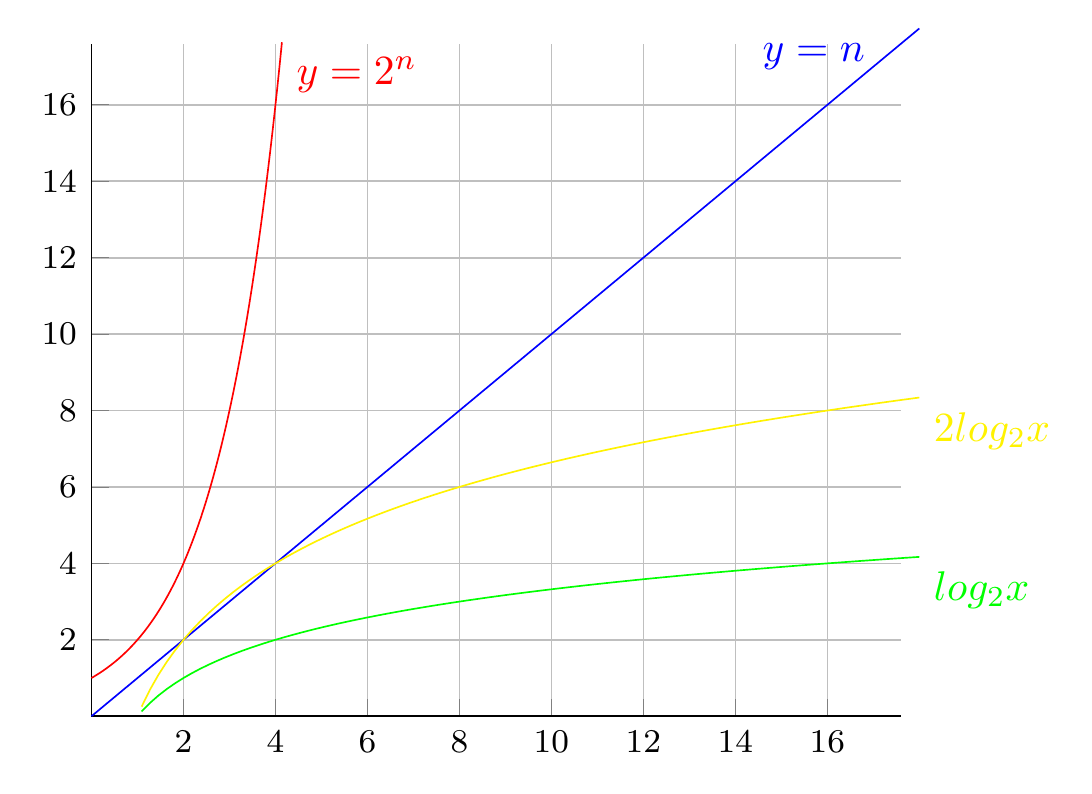
\begin{tikzpicture}[scale=1.5, transform shape]
\begin{axis}[grid=both,
      mark = none,
      xmin = 0, ymin = 0,
      xmax = 16,ymax = 16,
      axis lines*=middle,
      enlargelimits=upper,
      clip=false,
      xtick={0,2,...,16},
      ytick={0,2,...,16}]
\addplot[red, domain=0:5,restrict y to domain=0:18, samples=100]  {pow(2,x)} node[right,anchor=north west]{$y=2^n$};
\addplot[blue, domain=0:18,restrict y to domain=0:18, samples=100]  {x} node[anchor=north east,inner xsep=3ex] {$y=n$};
\addplot[green, domain=0:18,restrict y to domain=0:18, samples=100]  {ln(x)/ln(2)} node[right,anchor=north west]{$log_2x$};
\addplot[yellow, domain=0:18,restrict y to domain=0:18, samples=100]  {2*(ln(x)/ln(2))} node[right,anchor=north west]{$2log_2x$};
\end{axis}
\end{tikzpicture}
\caption{Wykres dla funkcji: $y=n$, $y=2^n$, $y=log2(x)$, $y=2log2(x)$}
\end{figure}

Dzieje się tak ze względu na to, że działanie algorytmów zależy od kolejności elementów w tablicy wejściowej, a nie od ich konkretnej wartości. W przypadku średnim, procedura tworzy mieszankę "dobrych" i "złych" podziałów.
\subsection{Najgorszy przypadek}
Istnieje też druga strona medalu i przypadek najgorszy. Następuje on, gdy podziały są maksymalnie niezrównoważone i za każdym razem tablica jest dzielona na dwie podtablice zawierające odpowiednio $n-1$ oraz 0 elementów. Wtedy koszt jednego podziału wynosi $\theta (n)$. Opisuje to rekurencyjne równanie: \\
\\
$T(n) = T(n-1) + T(0) + \theta(n) = T(n-1) + \theta(n)$, gdzie: \\
\\
$T(n-1)$ to czas przejścia po tablicy z $n-1$ elementami, $T(0)$ to czas przejścia po tablicy z 0 elementami, a $\theta(n)$ to koszt podziału najbardziej niezrównoważonego, wtedy: \\
\\
$T(n-1) + \theta(n) = \theta(n^2)$ \\
\\
Co daje czas działania tak wolny jak sortowanie przez wstawianie.
\chapter{Implementacje}
\section{Implementacja w pseudokodzie}
\begin{Verbatim}
Quicksort(A, p, r):
if p < r
	q = partition(A, p, r)
	quicksort(A, p, q-1)
	quicksort(A, q+1, r)
\end{Verbatim}
A - tablica do sortowania\\
p - pierwszy element (zazwyczaj 1)\\
r - długość tablicy\\
\\
"Jeśli długość tablicy jest większa niż indeks pierwszego elementu, to do zmiennej q zapisz wynik procedury "partition" na podanej tablicy A (czyli indeks pivota), i dokonaj podziału dwóch utworzonych podtablic metodą quicksort"  
\section{Implementacja w Python}
\subsection{Quicksort}
\begin{Verbatim}
def quick_sort(lst, start, stop, fun):
    if start < stop:
        border = fun(lst, start, stop)
        quick_sort(lst, start, border - 1, fun)
        quick_sort(lst, border + 1, stop, fun)
\end{Verbatim}
Definiujemy funkcję quicksort, przyjmującą parametry:
\begin{itemize}
\item lst - lista, którą będziemy sortować
\item start - punkt początkowy (start iteracji)
\item stop - punkt końcowy (koniec iteracji)
\item fun - funkcja wyboru pivota (wybierana spośród czterech: element pierwszy z lewej, ostatni z lewej, losowy, lub o środkowej wartości spośród elementów o indeksie pierwszym, środkowym i ostatnim)
\end{itemize}
Blok "if" warunkuje, że ostatni element na liście ma większy indeks niż element pierwszy. Po spełnieniu tego warunku do zmiennej "border" zapisujemy wartość, którą zwraca nam funkcja wyboru pivota działająca na parametrach: lista, start, stop; tak więc zostaje zwrócony indeks pivota, po czym przystępujemy do podziału tablicy na dwie podtablice, każda jest sortowana osobnym, rekurencyjnym wywołaniem quicksort.
\subsection{Partition}
\begin{Verbatim}
def partition(lst, start, stop):
    pivot_index = stop
    pivot_value = lst[pivot_index]
    for i in range(start, stop):
        if lst[i] < pivot_value:
            lst[i], lst[start] = lst[start], lst[i]
            start += 1
    lst[stop], lst[start] = lst[start], lst[stop]
    return start
\end{Verbatim}
\newpage
\subsection{Funkcje wyboru pivota}
\begin{Verbatim}
def partition_last(lst, start, stop):
    lst[stop], lst[stop] = lst[stop], lst[stop]
    return partition(lst, start, stop)
\end{Verbatim}
\textbf{Partition last} - pivot wybierany jako ostatni element listy.
\begin{Verbatim}
def partition_rand(lst, start, stop):
    rand_pivot = random.randint(start, stop)
    lst[stop], lst[rand_pivot] = lst[rand_pivot], lst[stop]
    return partition(lst, start, stop)
\end{Verbatim}
\textbf{Partition rand} - pivot wybierany jako losowy element listy.
\begin{Verbatim}
def partition_first(lst, start, stop):
    lst[stop], lst[start] = lst[start], lst[stop]
    return partition(lst, start, stop)
\end{Verbatim}
\textbf{Partition last} - pivot wybierany jako pierwszy element listy.
\begin{Verbatim}
def partition_middle(lst, start, stop):
    med = (len(lst)) // 2
    lst[stop], lst[med] = lst[med], lst[stop]
    return partition(lst, start, stop)
\end{Verbatim}
\textbf{Partition last} - pivot wybierany jako środkowy element listy.
\chapter{Testy i porównania}
\section{Testy}


\section{Porównanie z innymi algorytmami sortującymi}
\section{Bibliografia}
\end{document}
